% ============================================================
%  深圳大学实验报告模板（SZU Experiment Report Template）
%  Original: Chao Fan and Kewei Ou, AI School of SZU
%  https://github.com/ChaoFan996/Experiment-Report-Template-SZU
%  Modified for Project 1: NumPy implementation of OpenCLIP ViT-B/32.
%  Compile on Overleaf with XeLaTeX (Noto Serif CJK SC is bundled).
% ============================================================

\documentclass[a4paper,12pt]{article}

% ----------------------------
% 中文与字体支持
% ----------------------------
\usepackage{fontspec}
\usepackage{xeCJK}
\setCJKmainfont{Noto Serif CJK SC}

% ----------------------------
% 页面设置与常用宏包
% ----------------------------
\usepackage{geometry}
\geometry{left=0.9in, right=0.9in, top=0.85in, bottom=0.85in}
\usepackage{longtable}
\usepackage{graphicx}
\usepackage{fancyhdr}
\usepackage{tikz}
\usetikzlibrary{calc}
\usepackage{verbatim}
\usepackage{float}
\usepackage{booktabs}
\usepackage{xcolor}
\usepackage{hyperref}
\hypersetup{colorlinks=true, urlcolor=blue!60!black}

% 红色高亮（课程要求 Highlight Your Parts in RED）
\newcommand{\hl}[1]{\textcolor{red!85!black}{\textbf{#1}}}
\newcommand{\code}[1]{\texttt{\small #1}}
\setlength{\parindent}{0pt}
\setlength{\parskip}{5pt}

\fancyhf{}
\fancyhead[C]{}
\fancyhead[R]{}

% ============================================================
%                      文档开始
% ============================================================
\begin{document}

% ============================================================
% 封面页
% ============================================================
\begin{titlepage}
    \centering
    \vspace*{2cm}
    \Huge{\textbf{深 \ 圳 \ 大 \ 学 \ 实 \ 验 \ 报 \ 告}}\\[1.5cm]

    {\Large\textbf{课程名称}\quad\underline{\makebox[8cm][c]{Python程序设计}}}\\[0.5cm]
    {\Large
    \noindent\makebox[3.2cm][l]{\textbf{项目名称}}
    \underline{\makebox[8cm][c]{Project 1: NumPy 图像编码器}}}\\[0.5cm]
    {\Large
    \noindent\makebox[3.2cm][l]{\textbf{学 \quad \quad 院}}
    \underline{\makebox[8cm][c]{人工智能学院}}}\\[0.5cm]
    {\Large
    \noindent\makebox[3.2cm][l]{\textbf{专 \quad \quad 业}}
    \underline{\makebox[8cm][c]{人工智能}}}\\[0.5cm]
    {\Large
    \noindent\makebox[3.2cm][l]{\textbf{指导教师}}
    \underline{\makebox[8cm][c]{舒婷}}}\\[0.5cm]
    {\Large
    \noindent\makebox[3.2cm][l]{\textbf{报 \quad 告 \quad 人}}
    \underline{\makebox[3cm][c]{陈思翰}}
    \hspace{0.5cm}
    \textbf{学号}
    \underline{\makebox[3cm][c]{}}}\\[0.5cm]
    {\Large
    \noindent\makebox[3.2cm][l]{\textbf{实验时间}}
    \underline{\makebox[8cm][c]{2026-11-22}}}\\[0.5cm]
    {\Large
    \noindent\makebox[3.2cm][l]{\textbf{提交时间}}
    \underline{\makebox[8cm][c]{}}}\\[1.2cm]

    {\normalsize GitHub: \url{https://github.com/Chen-zzz123/Project1-NumPy-ImageEncoder}\par}
    \vfill
    \Large{\textbf{教务处制}}
\end{titlepage}

\newpage

% ============================================================
% 正文部分
% ============================================================
\section{Objectives}

本实验的目标是在\textbf{不使用 PyTorch、不训练、不联网}的条件下，仅用 NumPy 复现 OpenCLIP ViT-B/32 图像塔的完整前向计算，使其输出与课程提供的独立 FP32 参考结果在数值容差内一致。课程提供 152 个已训练权重张量；输入为预处理后的 \code{[B,3,224,224]} 图像，输出为 \code{[B,512]} 的单位长度语义向量。该编码器后续将作为 final project 中 \code{szu\_python\_openclip} 的图像塔复用。

\vspace{2pt}
\noindent\colorbox{red!6}{\parbox{\dimexpr\linewidth-2\fboxsep\relax}{
\textcolor{red!85!black}{\textbf{【本人完成的核心工作】}} 独立完成 \code{image\_encoder.py} 中全部 \hl{6 组 TODO} 的 NumPy 实现：\hl{patchify 的 6 维轴重排}、\hl{多头注意力的分头/合头与 4D 转置}、\hl{12 层残差与 MLP}、\hl{图块投影与 CLS/位置编码}、\hl{CLS 后置 Norm 与 512 维输出头}；逐阶段运行 \code{check.py} 定位误差，并\hl{修复了一处真实的轴转置 bug}（第 5 节）。}}

\section{Overview}

ViT 的思路是``把图片当句子''：先把 $224\times224$ 图片切成 $7\times7=49$ 个 $32\times32$ 图块，每块摊平成 3072 个数；用无偏置线性层压成 768 维 token；最前面拼一个可学习的 CLS``摘要行''并加位置编码，得到 50 行 token；让 12 个 Transformer 块反复提炼（形状不变）；最后只取 CLS 行，经后置 LayerNorm、512 维投影与单位长度归一化，得到图片的语义向量。

\begin{figure}[H]
    \centering
    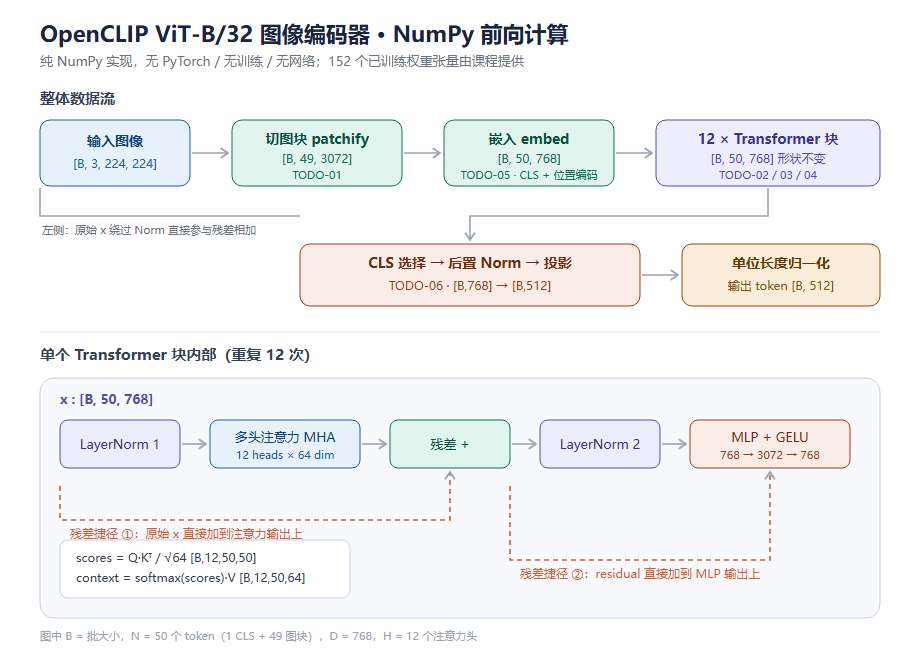
\includegraphics[width=0.98\linewidth]{figs/vit_overview.png}
    \caption{整体数据流与单个 Transformer 块内部结构；橙色虚线为两条残差捷径。}
    \label{fig:vit-arch}
\end{figure}

如 Figure~\ref{fig:vit-arch} 所示，每个 Transformer 块包含两次残差相加：\code{residual = x + attn(norm1(x))} 与 \code{output = residual + MLP(norm2(residual))}。三个必须记住的模型约定：
\begin{enumerate}
    \item 线性层权重存为 \code{[out,in]}，故用 \code{W.T}；\hl{唯一例外 \code{visual.proj} 已是 [in,out]=[768,512]，不可转置}。
    \item 真实 \code{k} 是 4D \code{[B,12,50,64]}，只能 \code{transpose(0,1,3,2)} 交换最后两轴，不能整体 \code{.T}。
    \item 图块投影与最终投影均无偏置；GELU 必须用课程提供的精确 \code{erf} 版本；全程保持 float32。
\end{enumerate}

\section{Implementations}

\begin{table}[H]
\centering\small
\begin{tabular}{@{}l l l@{}}
\toprule
TODO & 关键操作 & 形状变化\\
\midrule
01 \code{patchify} & \code{reshape} $\to$ \code{transpose(0,2,4,1,3,5)} $\to$ \code{reshape} & \code{[B,3,224,224]} $\to$ \code{[B,49,3072]}\\
02 \code{split\_heads} & \code{reshape(B,N,12,64).transpose(0,2,1,3)} & \code{[B,N,768]} $\to$ \code{[B,12,N,64]}\\
03 MHA & \code{QK$^\mathsf{T}/\sqrt{64}$} $\to$ softmax $\to$ \code{@V} $\to$ 合头 $\to$ 投影 & \code{[B,12,50,50]} $\to$ \code{[B,50,768]}\\
04 Block & 两次残差相加 + \code{GELU(uW1+b1)W2+b2} & \code{[B,50,768]} 不变\\
05 \code{embed} & \code{patches @ W.T} + 拼 CLS + \code{+ position} & \code{[B,49,3072]} $\to$ \code{[B,50,768]}\\
06 \code{\_\_call\_\_} & 取 CLS $\to$ \code{post\_norm} $\to$ \code{@ proj} $\to$ \code{unit\_vector} & \code{[B,50,768]} $\to$ \code{[B,512]}\\
\bottomrule
\end{tabular}
\end{table}

\hl{分头时采用 \code{reshape(B,N,12,64)} 而非按头分块后再排}，因为 PyTorch 的 \code{in\_proj\_weight} 按``头是外层循环''的顺序拼接，该顺序由 \code{block0} 阶段独立验证。代码内每个 TODO 均附逐步形状注释，可对照 \code{PPT-CODE-MAP.txt} 的幻灯片 39--70 页阅读。

\section{Results}

复现命令：\code{python check.py --stage all}（原始输出见 \code{report/check\_results.txt}，约 10 秒）。

\begin{table}[H]
\centering\small
\begin{tabular}{@{}l l r r l l@{}}
\toprule
Stage & Shape & max abs err & mean abs err & 容差 atol/rtol & 结果\\
\midrule
preprocess   & (10,3,224,224) & 0.000e+00 & 0.000e+00 & 2e-6 / 2e-4 & PASS\\
patches      & (2,49,3072)    & 0.000e+00 & 0.000e+00 & 2e-4 / 2e-4 & PASS\\
tokens       & (2,50,768)     & 4.005e-05 & 1.289e-06 & 2e-4 / 2e-4 & PASS\\
block0       & (2,50,768)     & 7.063e-06 & 3.250e-07 & 2e-4 / 2e-4 & PASS\\
last\_tokens & (2,50,768)     & 4.768e-05 & 2.696e-06 & 2e-4 / 2e-4 & PASS\\
\textbf{output} & \textbf{(10,512)} & \hl{5.439e-07} & \hl{8.311e-08} & 2e-5 / 2e-4 & \textbf{PASS}\\
\textbf{batch}  & \textbf{(3,512)}  & \hl{4.619e-07} & \hl{7.632e-08} & 2e-5 / 2e-4 & \textbf{PASS}\\
\bottomrule
\end{tabular}
\end{table}

\code{preprocess} 与 \code{patches} 误差为 0，说明重排类操作与 Torch 完全一致；\code{tokens} 之后的 1e-5 量级误差来自 NumPy 与 Torch 在矩阵乘累加顺序上的浮点舍入差异，经过 12 层后未放大，最终输出收敛到 5e-7。\code{batch} 阶段用 \code{[1,0,1]} 打乱顺序并重复图片，验证实现不依赖固定 batch 大小、不缓存参考行。\code{run.py} 另生成 10 张图的 \code{(10,512)} float32 输出，每行 L2 范数均为 1.000。

\noindent\hl{结论：全部 8 个阶段 PASS}，最大输出误差比容差小约两个数量级。

\section{Discussion}

\textbf{一次形状变换：patchify 的 6 维轴重排。} 输入 \code{[B,3,224,224]} 要得到 \code{[B,49,3072]}，图块须``从左到右、再从上到下''排列，块内按 \code{C,H,W} 摊平。先把 224 拆成``7 个块 $\times$ 块内 32 像素''：
\begin{verbatim}
images.reshape(B, 3, 7, 32, 7, 32)      # B,C,row-block,row-in,col-block,col-in
      .transpose(0, 2, 4, 1, 3, 5)     # B,row-block,col-block,C,row-in,col-in
      .reshape(B, 49, 3072)            # 49 = 7*7; 3072 = 3*32*32
\end{verbatim}
\code{transpose(0,2,4,1,3,5)} 把行/列块号提到最前，保证 \code{(row,col)} 行优先；把 \code{C,行内,列内} 留在最后，保证摊平顺序 \code{C$\to$H$\to$W}。若误写成 \code{(0,3,5,1,2,4)}，图块顺序变为列优先，\code{patches} 阶段会立刻 FAIL。\hl{\code{reshape} 只按内存顺序重新分组、不改变元素相对次序，只有 \code{transpose} 能真正交换轴}。

\textbf{一个真实修复的 bug。} 实现 TODO-03a 时沿用课堂 2D 算例的写法 \code{scores = (q @ k.T) / scale}，运行 \code{--stage block0} 报：
\begin{verbatim}
block0 FAIL: matmul: Input operand 1 has a mismatch in its
core dimension 0, with gufunc signature (n?,k),(k,m?)->(n?,m?)
(size 12 is different from 64)
\end{verbatim}
课堂 \code{k} 是 2D，\code{.T} 只交换两个轴；真实 \code{k} 是 4D \code{[B,12,50,64]}，\code{.T} 会把所有轴反转成 \code{[64,50,12,B]}，导致核心维度 12 与 64 对不上。改为 \code{k.transpose(0,1,3,2)} 后 \hl{PASS（max\_abs=7.063e-06）}。通用规律：从 2D 教学代码迁移到 4D 批量代码时，任何 \code{.T} 都要显式写成 \code{transpose} 并核对轴编号。

\textbf{贡献与外部协助（如实声明）。} 本次作业在 AI 助手（WorkBuddy，腾讯混元模型）协助下完成：AI 提供六个 TODO 的实现思路与代码骨架、逐行形状注释、架构插图、README 与本报告排版。\hl{本人完成的部分}：核对每个公式与权重方向约定、运行全部 \code{check.py} 阶段验证、执行上述错误注入与修复实验、整理误差表格与结论。课程提供的 \code{helpers.py} / \code{check.py} / \code{run.py} 等文件均未修改，参考输出从未作为编码器输入。

\textbf{复现}：\code{python -m pip install -r requirements.txt} $\to$ \code{python check.py --stage all} $\to$ \code{python run.py --output output\_tokens.npz}。完整步骤与 GitHub 链接见仓库 \code{README.md}。

\newpage

% ============================================================
% 批阅与成绩评定页（模板自带，供教师使用）
% ============================================================
\begin{tikzpicture}[remember picture, overlay]
  \draw[thick]
    ($(current page.north west)+(2cm,-3cm)$)
    rectangle
    ($(current page.south east)+(-2cm,3.5cm)$);
\end{tikzpicture}

\vspace{1cm}
\noindent \textbf{指导教师批阅意见：}
\vspace{6cm}
\hfill
\vspace{1cm}
\noindent \textbf{成绩评定：}
\vspace{2cm}
\hfill
\vspace{1cm}
\noindent
\hfill
\textbf{指导教师签字：}\quad\quad\quad\quad\quad\\[0.5cm]
\hfill
\textbf{年}\quad\quad
\textbf{月}\quad\quad
\textbf{日}\quad
\vspace{1cm}
\noindent \textbf{备注：}

\begin{tikzpicture}[remember picture, overlay]
  \node[
    anchor=north west,
    inner sep=0pt,
    text width=\dimexpr\paperwidth-4cm\relax
  ] at ($(current page.south west)+(2cm,3.1cm)$) {
    \begin{minipage}{\dimexpr\paperwidth-4cm\relax}
      \small
      \noindent
      \textbf{注：}\;1、报告内的项目或内容设置，可根据实际情况加以调整和补充。\\[0.2cm]
      \phantom{\textbf{注：}\;}2、教师批改学生实验报告时间应在学生提交实验报告时间后 10 日内。
    \end{minipage}
  };
\end{tikzpicture}

\end{document}
